\chapter{Resultados e Análises}

% - OK Achei o texto introdutório um pouco fraco em apresentar o objetivo do capítulo. 
% 	OK	Acho que vocês poderia focar primeiro que os testes foram para identificar a acurácia do sistema perante seus requisitos (Identificação e Localização). 
% OK		Apresentar o LAICO apenas como o local onde ocorreram os testes. 
% 		Apresentar cada ponto como uma medida/indicador do sistema desenvolvido. 
% 		OK No texto dos 4 testes foque nos objetivos e não no como. Tipo:
% 			Rastreamento: Testar a acurácia do rastreamento e identificação de objetos em situações do cotidiano.
% 			Reconhecimento: Testar a acurácia de identificação dos usuários perante a base de dados.

	Com intuito de identificar a acurácia e as limitações do Sistema TRUE perante seus requisitos (identificação, rastreamento e localização) foram feitos uma série de testes funcionais. Grande parte dos testes foram realizados no LAICO (\textbf{LA}boratório de Sistemas \textbf{I}ntegrados e \textbf{CO}ncorrente), um laboratório do Departamento de Ciência da Computação da Universidade de Brasília. 

	% O LAICO possui dimensões de $\displaystyle 7,67m$ x $\displaystyle 6,45m$ ilustrado pela Figura~\ref{fig:laico}.

	% \begin{figure}[htb]
	% 		\begin{center}
	% 			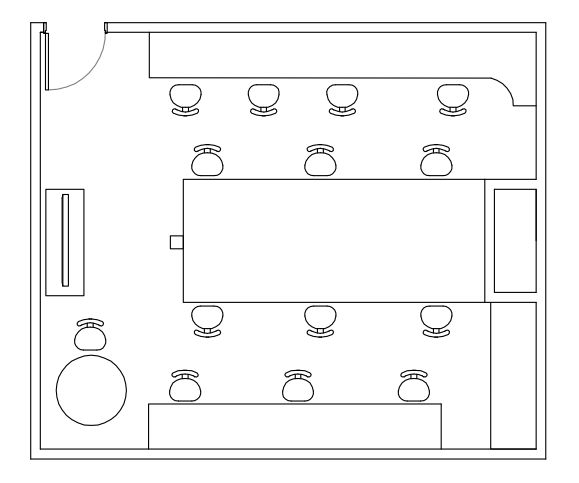
\includegraphics[scale=0.6]{figuras/4.ProblemaEProposta/laico.png}
	% 		\end{center}
	% 		\caption{Planta do \textit{SmartSpace} Laico.}
	% 		\label{fig:laico}
	% 	\end{figure}	

	Cada teste tinha como foco um das funcionalidades do Sistema TRUE:

	\begin{itemize}
		\item \textbf{Rastreamento}: testes funcionais realizados para avaliar a eficiência da detecção de novos usuários e que simulam diferentes situações diárias mostrando como o sistema se comporta quando ocorre oclusões parciais e totais de usuários e quando os mesmos interagem entre si ou com objetos no ambiente.

		\item \textbf{Reconhecimento}: testes realizados para avaliar a acurácia na identificação do usuários perante uma base de dados.

		% diferentes pessoas foram cadastradas no sistema e reconhecidas pelo mesmo. As diferentes identidades obtidas em cada reconhecimento foram inseridas em uma matriz de confusão para avaliar a acurácia do reconhecimento.

		\item \textbf{Localização}: testes realizados para avaliar a precisão do sistema ao estimar a posição dos usuários no ambiente.
	% um objeto foi colocado no ambiente em diferentes posições pre-determinadas e as coordenadas obtidas pelo sistema foram inseridas em gráficos e foram comparadas com as coordeanadas reais avaliando a precisão do sistema.

		\item \textbf{Integração com o middleware \textit{UbiquitOS}}: uma aplicação foi desenvolvida para testar a integração do Sistema TRUE com o middleware \textit{UbiquitOS}, testando os serviços disponíveis e os eventos gerados.

		% uma aplicação foi desenvolvida para o middleware \textit{UbiquitOS}. Ela consome alguns serviços e eventos produzidos pelo driver \textit{UserDriver} que são comparados com as informações reais.
	\end{itemize}

\section{Rastreamento dos Usuários}

	O rastreamento é fundamental para o funcionamento correto do sistema uma vez que é responsável por rastrear os usuários no ambiente, determinar a sua localização física em relação ao sensor \textit{Kinect} e gerenciar suas identidades. Portanto, foi realizado uma série de testes funcionais para determinar suas limitações.

	Os primeiros testes realizados foram para testar a eficiência da detecção de novos usuários no ambiente. Os testes foram feitos simulando a entrada de um usuário na cena por diferentes ângulos e analisando o momento em que o mesmo era detectado. Em todos os testes o usuário era detectado antes mesmo de entrar na área de visão do sistema por completo, como mostrado na Figura~\ref{fig:testes_deteccao}.
	
		\begin{figure}[htb]
			\begin{center}
				\subfloat[] {
					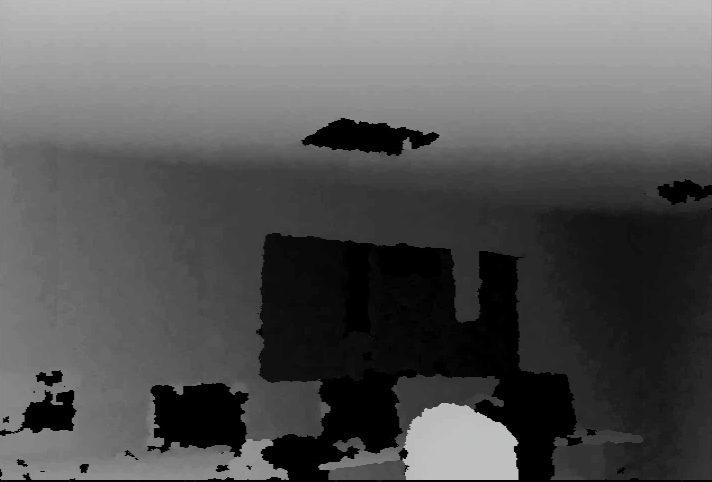
\includegraphics[width=0.25\textwidth]{figuras/5.Testes/deteccao/1.png}}
				\subfloat[] {
					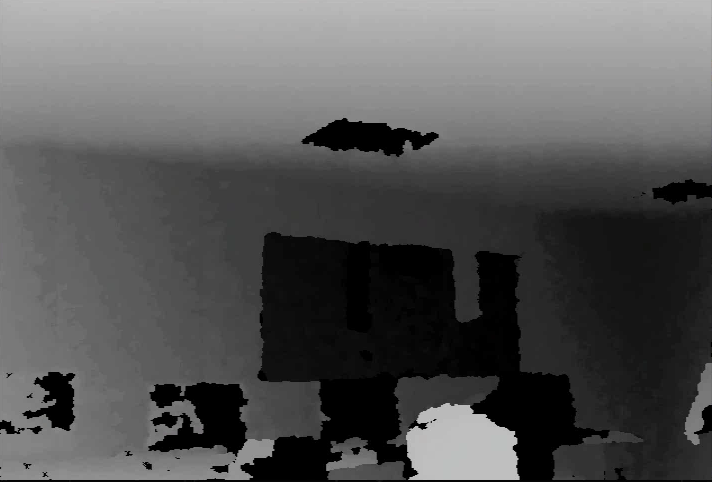
\includegraphics[width=0.25\textwidth]{figuras/5.Testes/deteccao/2.png}}
				\subfloat[] {
					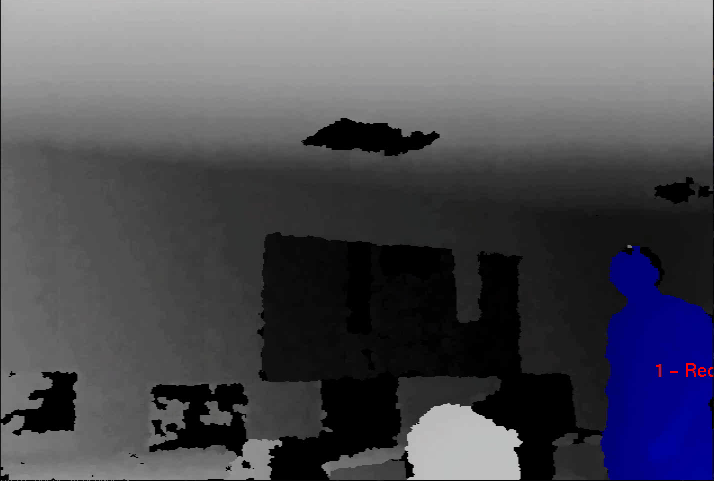
\includegraphics[width=0.25\textwidth]{figuras/5.Testes/deteccao/3.png}}
				\subfloat[] {
					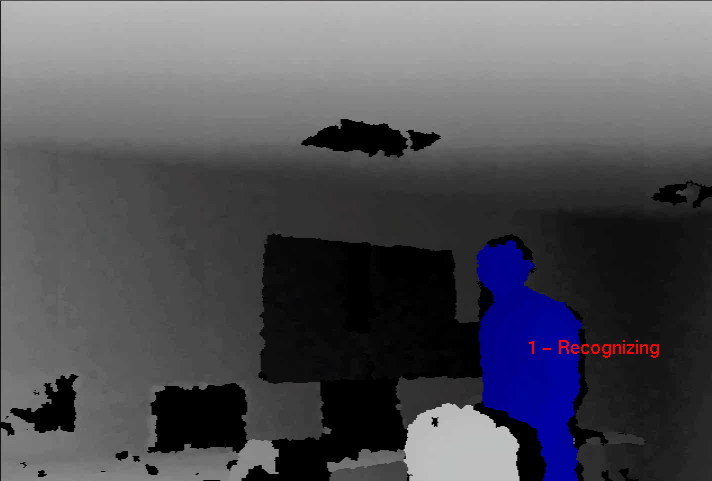
\includegraphics[width=0.25\textwidth]{figuras/5.Testes/deteccao/4.png}}
			\end{center}
			\caption{Momento em que um novo usuário foi detectado pelo Sistema TRUE.}
			\label{fig:testes_deteccao}
		\end{figure}

	Também foram realizados testes para tentar avaliar o impacto da oclusão no rastreamento. Em alguns testes um usuário se posicionava no ambiente com intuito de ocultar totalmente outro usuário rastreado. Com isso, caso o usuário continuasse oculto, o sistema o dava como perdido. Porém, o sistema se mostrou robusto em casos que a oclusão era parcial, como mostrado na Figura~\ref{fig:testes_oclusao_sucesso} Em outros testes, foi simulada uma situação mais comum: quando um usuário, em movimento, ocultava ou era oculto, por um momento, por outro usuário. Neste caso, o sistema logo conseguia se recuperar e voltar a rastrear o usuário perdido, como mostrado na Figura~\ref{fig:testes_oclusao}. A oclusão era um problema esperado pois o Sistema TRUE utiliza somente um sensor \textit{Kinect} como dispositivo de entrada.
		
		\begin{figure}[htb]
			\begin{center}
				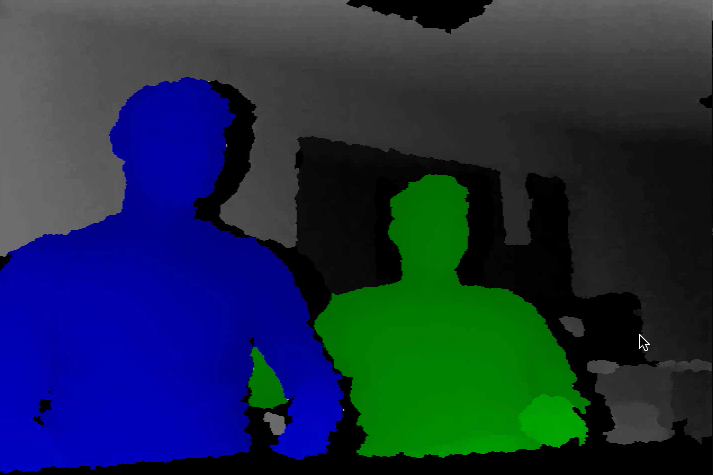
\includegraphics[width=0.75\textwidth]{figuras/5.Testes/oclusao/oclusao_corretamente.png}
			\end{center}
			\caption{Oclusão parcial de dois usuários.}
			\label{fig:testes_oclusao_sucesso}
		\end{figure}
	
		\begin{figure}[htb]
		\begin{center}
				\subfloat[] {
					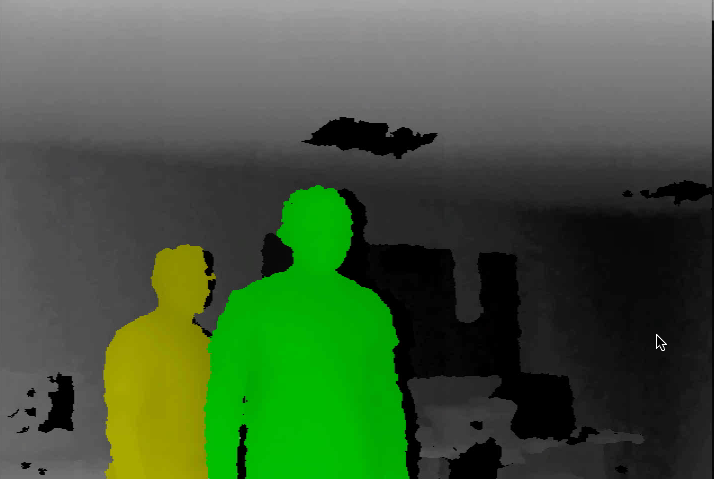
\includegraphics[width=0.19\textwidth]{figuras/5.Testes/oclusao/1.png}}
				\subfloat[] {
					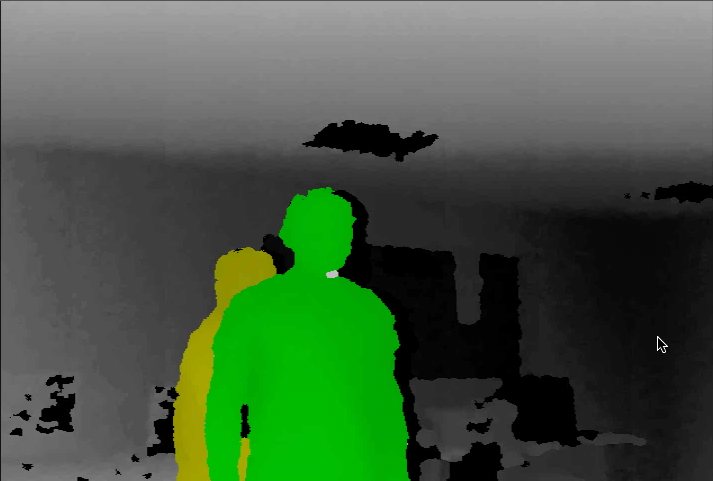
\includegraphics[width=0.19\textwidth]{figuras/5.Testes/oclusao/2.png}}
				\subfloat[] {
					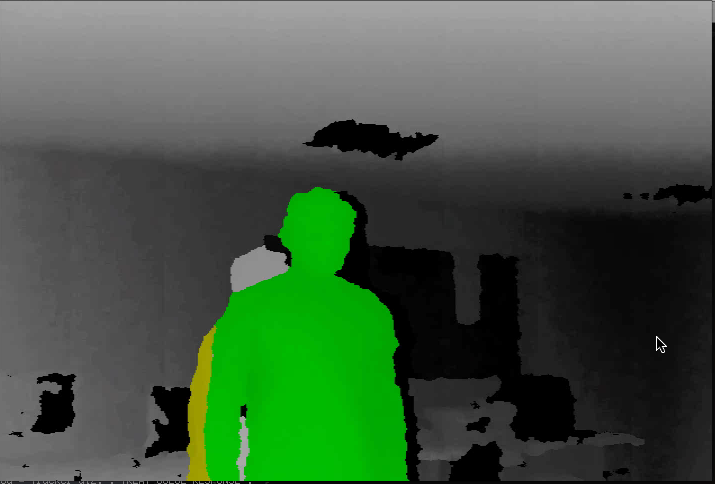
\includegraphics[width=0.19\textwidth]{figuras/5.Testes/oclusao/3.png}}
				\subfloat[] {
					\label{fig:testes_oclusao_ocluso}
					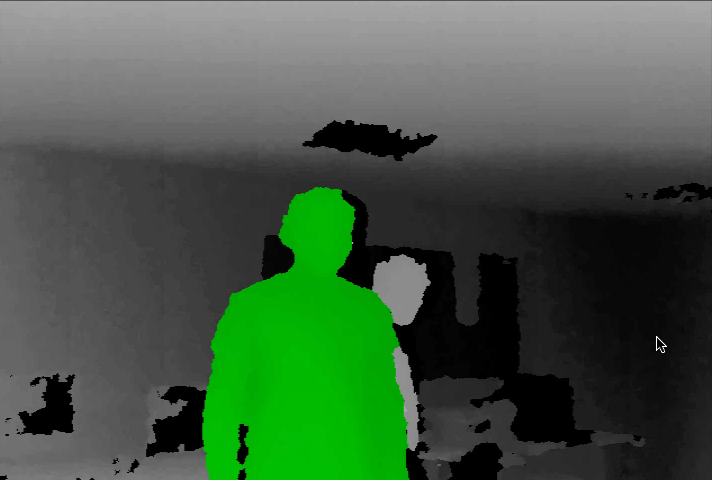
\includegraphics[width=0.19\textwidth]{figuras/5.Testes/oclusao/4.png}}
				\subfloat[] {
					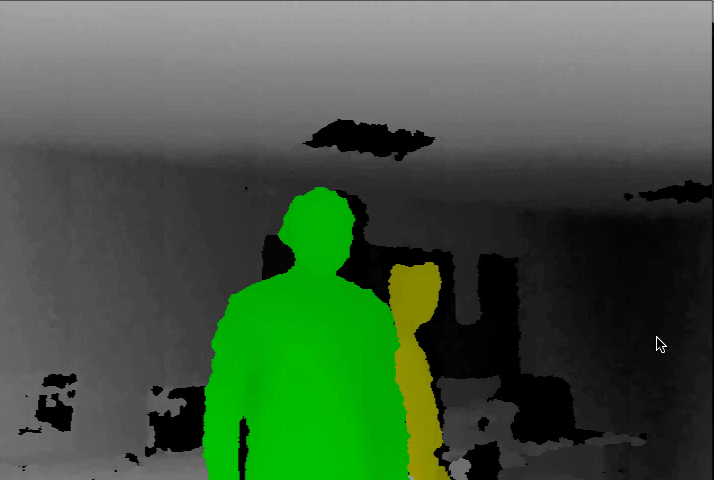
\includegraphics[width=0.19\textwidth]{figuras/5.Testes/oclusao/5.png}}
			\end{center}
			\caption{Oclusão de usuários.}
			\label{fig:testes_oclusao}
		\end{figure}

	Outra caracterísitca importante que foi testada é a abrangência do campo de
	visão do Sistema TRUE. Como já mensionado o sistema utiliza o sensor
	\textit{Kinect} que possui um campo de visão horizontal de 57º. Então, a uma
	distância de, aproximadamente, 4 metros do sensor, o número máximo de usuários
	que cabem no campo de visão sem que haja oclusão são 5 pessoas, como mostrado
	na Figura~\ref{fig:max-pessoas}.

	\begin{figure}[htb]
			\begin{center}
				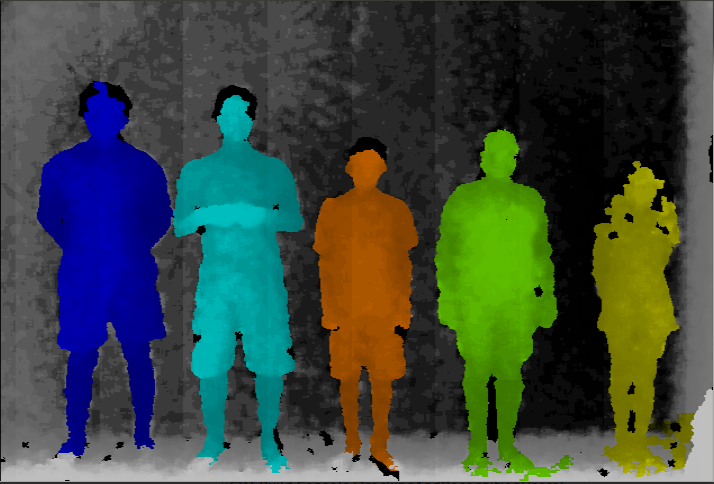
\includegraphics[width=0.4\textwidth]{figuras/5.Testes/oclusao/max-pessoas.png}
			\end{center}
			\caption{Usuários posicionados lado a lado do sensor \textit{Kinect} a uma distância de 4 metros.}
			\label{fig:max-pessoas}
		\end{figure}
		
	Durante os testes realizados com rastreamento foi observado alguns problemas que ocorriam quando o usuário rastreado interagia com objetos ou com outros usuários. Na grande parte das vezes que o usuário interagia com objetos, o Sistema TRUE considerava o objeto como sendo parte do usuário como exemplificado na Figura~\ref{fig:testes_relacionamento_com_objetos}, o que não prejudicou a eficiência do sistema. Já os problemas com interação entre usuários eram bem mais raros, porém o impacto era maior. Esses problemas consistem em algumas ``interferências'' que podiam acontecer quando havia contato entre dois ou mais usuários. A Figura~\ref{fig:testes_relacionamento_com_usuarios} exemplifica melhor essas ``interferências''.
	
		\begin{figure}[htb]
			\begin{center}
				\subfloat[] {
					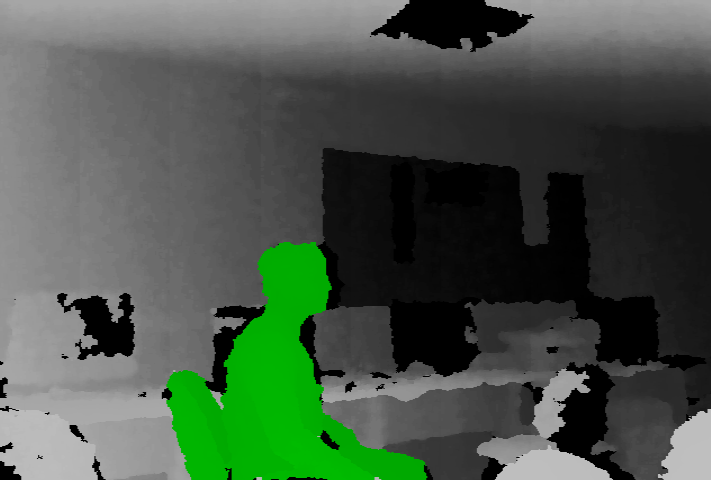
\includegraphics[width=0.37\textwidth]{figuras/5.Testes/relacionamento_com_objetos/1.png}}
				\subfloat[] {
					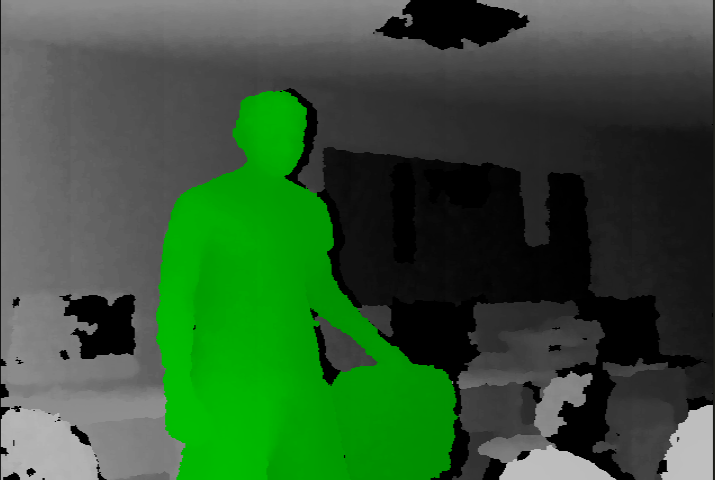
\includegraphics[width=0.37\textwidth]{figuras/5.Testes/relacionamento_com_objetos/2.png}}
			\end{center}
			\caption{Usuários sendo rastreado conjuntamente com os objetos que
			interagem.}
			\label{fig:testes_relacionamento_com_objetos}
		\end{figure}
		
		\begin{figure}[htb]
			\begin{center}
				\subfloat[] {
					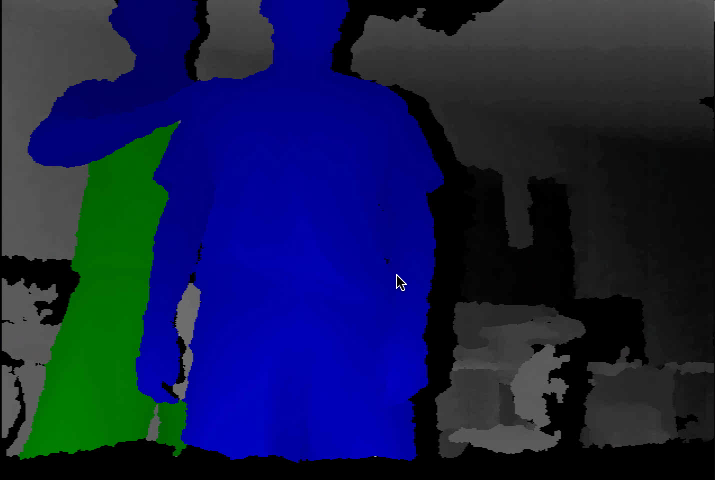
\includegraphics[width=0.32\textwidth]{figuras/5.Testes/relacionamento_com_pessoas/1.png}}
				\subfloat[] {
					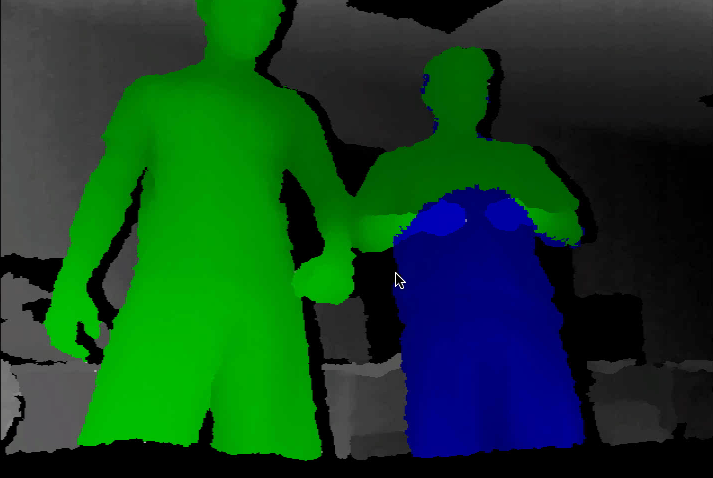
\includegraphics[width=0.32\textwidth]{figuras/5.Testes/relacionamento_com_pessoas/2.png}}
				\subfloat[] {
					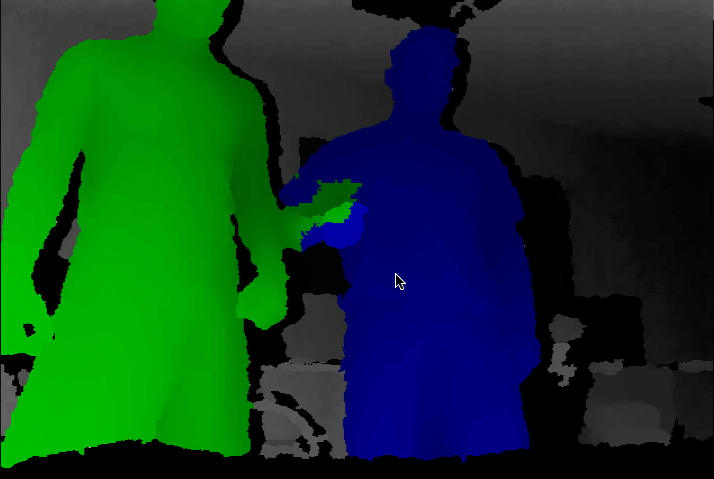
\includegraphics[width=0.32\textwidth]{figuras/5.Testes/relacionamento_com_pessoas/3.png}}
			\end{center}
			\caption{Usuários sofrendo interferência dos que estão ao seu redor.}
			\label{fig:testes_relacionamento_com_usuarios}
		\end{figure}

	Apesar dos problemas relatados, o rastreamento conseguiu, na maioria dos testes, atender as necessidades rastreando os diversos usuários no ambiente em suas atividades diárias, como mostrado na Figura~\ref{fig:varios-usuarios-ambiente}.

		\begin{figure}[htb]
			\begin{center}
				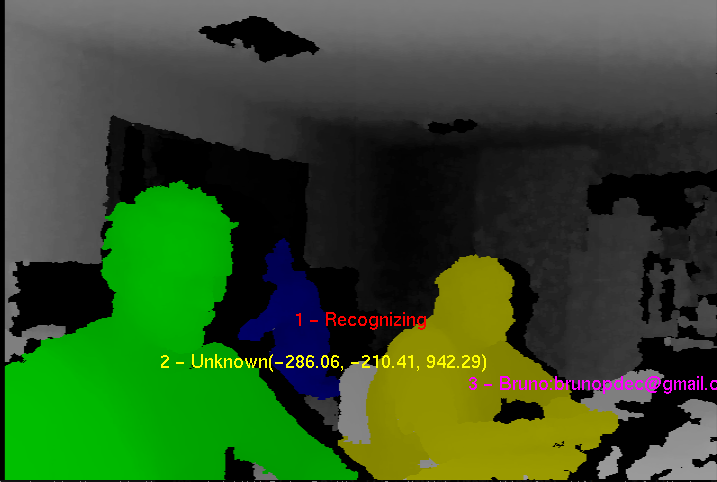
\includegraphics[scale=0.5]{figuras/5.Testes/oclusao/usuarios-rastreados.png}
			\end{center}
			\caption{Usuários rastreados pelo Sistema TRUE.}
			\label{fig:varios-usuarios-ambiente}
		\end{figure}
		
	

\section{Localização dos Usuários}

O Sistema TRUE obtém a localização dos usuários no ambiente por meio de coordenadas dos mesmos em relação ao \textit{Kinect}. Para saber o quanto essas coordenadas são confiáveis foram realizados alguns testes que resultaram em gráficos que comparam as coordenadas obtidas pelo sistema e as coordenadas reais.

As coordenadas $\displaystyle (x, y, z)$ obtidas pelo sistema são coordenas de um plano cartesiano de três dimensões em que o ponto $\displaystyle (0, 0, 0)$ corresponde a posição do \textit{Kinect}. Os valores das coordenadas que realmente são utilizadas para estimar a localização do usuário no ambiente são os valores nos eixos $\displaystyle x$ e $\displaystyle z$. Os valores do eixo $\displaystyle y$ correspondem somente a altura do centro de massa geométrico do usuário rastreado. Portanto, os testes desenvolvidos aferiram somente os valores obtidos pelo Sistema TRUE nos eixos $\displaystyle x$ e $\displaystyle z$.

\subsection{Teste dos valores no eixo $\displaystyle z$}

	Os valores obtidos no eixo $\displaystyle z$ correspondem aos valores de profundidade do usuário rastreado em relação ao \textit{Kinect}. Portanto, para testar a precisão do Sistema TRUE foi realizado o seguinte teste: um objeto (uma caixa de papelão) foi colocada em frente ao sensor, como mostrado na Figura~\ref{fig:teste-z}, em diferentes distâncias do mesmo (1 metro, 2 metros, 3 metros, 4 metros, 4,057 metros). Para cada distância, foram anotados alguns valores obtidos pelo sistema, mostrados na Tabela~\ref{tab:valores-z}, e foram obtidas diferentes imagens do Sistema TRUE mostradas na Figura~\ref{fig:distancias}. Então esses valores foram inseridos em um gráfico e comparado com os valores reais.

	\begin{figure}[htb]
		\begin{center}
			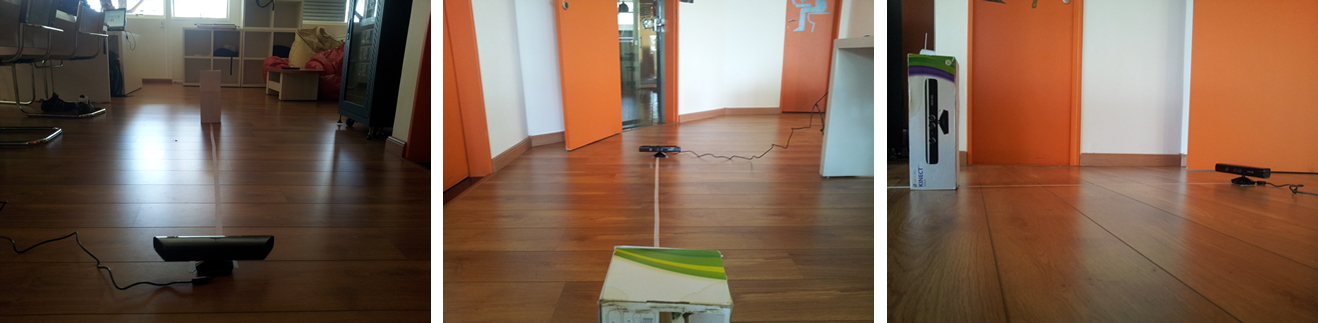
\includegraphics[scale=0.35]{figuras/5.Testes/teste-eixoz.png}
		\end{center}
		\caption{Fotos retiradas no teste realizado para aferir os valores obtidos no eixo $\displaystyle z$.}
		\label{fig:teste-z}
	\end{figure}

	\begin{figure}[htb]
		\begin{center}
			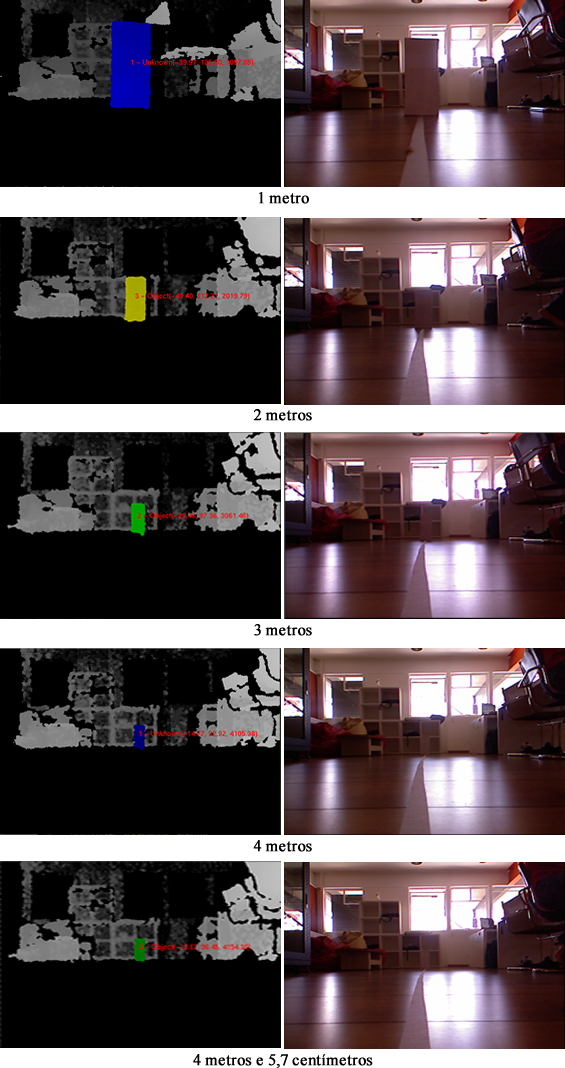
\includegraphics[scale=0.6]{figuras/5.Testes/eixoz-imgs.png}
		\end{center}
		\caption{Fotos retiradas no teste realizado para aferir os valores obtidos no eixo $\displaystyle z$.}
		\label{fig:distancias}
	\end{figure}

		\begin{table}[h]
		\begin{center}
			\caption{Valores obtidos pelo Sistema TRUE.}
			\begin{tabular}{|c|c|c|c|c|}
				\hline \bf Distância do objeto ao \textit{Kinect} (mm) & \multicolumn{4}{|c|}{\bf Valores obtido pelo Sistema TRUE (mm)} \\
				\hline
				\hline 1000,00 & 1007,56 & 1006,64 & 1003,21 & 1007,56 \\
				\hline 2000,00 & 2020,27 & 2021,17 & 2020,55 & 2020,48 \\
				\hline 3000,00 & 3058,70 & 3057,60 & 3062,01 & 3059,10 \\
				\hline 4000,00 & 4115,31 & 4110,25 & 4111,59 & 4114,80 \\
				\hline 4057,00 & 4166,35 & 4163,83 & 4166,45 & 4168,75 \\
				\hline
			\end{tabular}
		\end{center}
		\label{tab:valores-z}
	\end{table}

	Os valores obtidos no teste foram inseridos em um gráfico representado pela Figura~\ref{fig:grafico-z}. Neste gráfico existem duas retas: uma reta preta que representa valores ideias que batem com os valores reais; e uma reta vermelha que representa os valores obtidos pelo sistema. Como observado, a medida que o objeto se afasta do \textit{Kinect} as diferenças entre os valores reais e os valores obtidos aumetam. Contudo, essa diferença é de poucos centímetros.

	\begin{figure}[htb]
		\begin{center}
			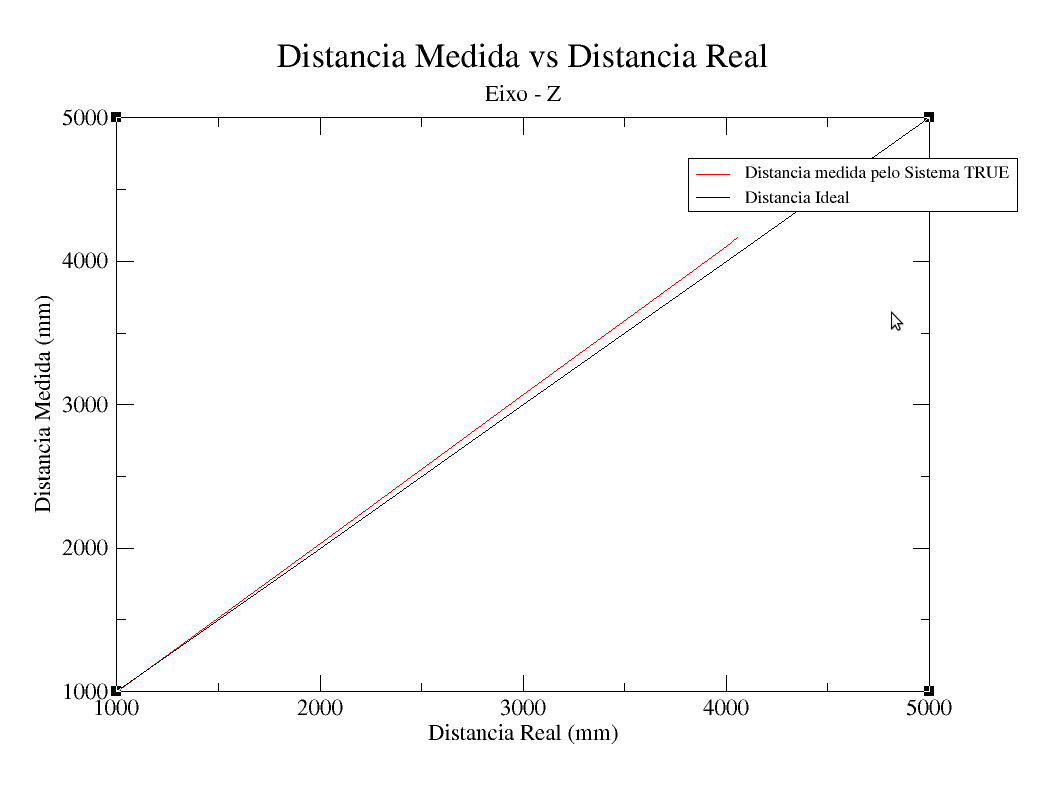
\includegraphics[scale=0.4]{figuras/5.Testes/grafico-eixo-z.png}
		\end{center}
		\caption{Gráfico comparativo entre os valores obtidos pelo Sistema TRUE e os valores reais.}
		\label{fig:grafico-z}
	\end{figure}

	Pelos resultados deste teste, pode-se concluir que o Sistema TRUE fornece informações sobre localização dos usuários bem precisas e confiáveis podendo ter erros de poucos centímetros que não prejudicam a integridade das informações. 

	Através deste teste, também foi possível obter a distância máxima e mínima que o usuário deve estar do \textit{Kinect} para que o sistema consiga rastrear-lo e estimar sua localização. A distância mínima é de $\displaystyle 48,3 cm$ e a máxima de $\displaystyle 4,057 m$.

\subsection{Teste dos valores no eixo $\displaystyle x$}



















\section{Identificação dos Usuários}
	
	Os usuários são identificados através do metodo conhecido como
	Eigenfaces~\ref{sec:reconhecimento}. Os usuários são identificados por suas
	labels de cadastro e a cada reconhecimento é associado a essa label uma
	confiança. Para validar a confiabilidade da identificação será usado a matriz
	de confusão para representar os dados dos testes.
	
	\begin{table}[H]
		\begin{center}
			\caption{Matriz de confusão para apresentar os resultados obtidos.}
			\begin{tabular}{|c|c|c|c|c|c|c|c|c|c|}
				\hline \bf X & \bf Tales & \bf Danilo & \bf Fabrício & \bf Ricardo & \bf
				Bruno & \bf Estevão & \bf Guto & \bf Tainá & \bf Tanyssa \\
				\hline \bf Tales & & & & & & & & & \\
				\hline \bf Danilo & & & & & & & & & \\
				\hline \bf Fabrício & & & & & & & & & \\
				\hline \bf Ricardo & & & & & & & & & \\
				\hline \bf Bruno & & & & & & & & & \\
				\hline \bf Estevão & & & & & & & & & \\
				\hline \bf Guto & & & & & & & & & \\
				\hline \bf Tainá & & & & & & & & & \\
				\hline \bf Tanyssa & & & & & & & & & \\
				\hline
			\end{tabular}
		\end{center}
		\label{tab:tabelaRequisitosTeoricos}
	\end{table}


\section{Integração com Middleware \textit{uOS}}

	A integração do Middleware \textit{uOS} com o Sistema TRUE consiste em um \textit{driver} desenvolvido para que ambos possam se comunicar. Este \textit{driver} foi nomeado de \textit{UserDriver} que foi apresentado na Seção~\ref{sec:modulo-integracao}. Com intuito de exemplificar a utilização do \textit{UserDriver} e testar a integração do Sistema TRUE com o middleware \textit{uOS} foi desenvolvido uma aplicação para o middleware chamada \textit{UserApp}. Esta aplicação registra um \textit{listener} para ``escutar'' os eventos do \textit{UserDriver} chamado \textit{UserListener}. 

	Como aplicação o \textit{UserApp} apenas se inscreve para receber os eventos gerados pelo \textit{UserDriver}. Já o \textit{UserListener}, como \textit{listener}, espera os eventos serem gerados e realiza duas análises: analisa o evento (novo usuário detectado, usuário perdido, ou reconhecimento realizado) e analisa quanto tempo cada usuário está parado no mesmo lugar.

		% \begin{figure}[hbt]
		% 	\begin{center}
		% 		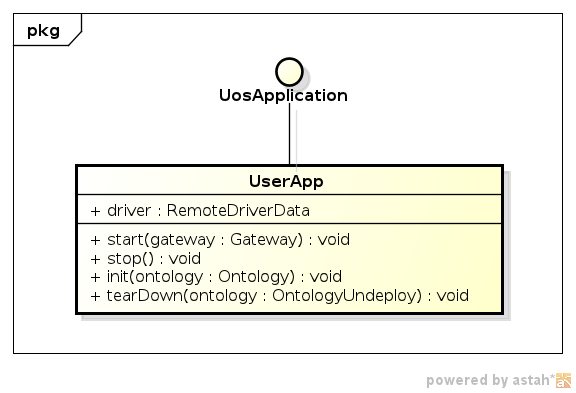
\includegraphics[scale=0.6]{figuras/5.Testes/diagrama-classe-user-ap.png}
		% 	\end{center}
		% 	\caption{Diagrama de Classe da aplicação \textit{UserApp}.}
		% 	\label{fig:diagrama-userapp}
		% \end{figure}

		% \begin{figure}[hbt]
		% 	\begin{center}
		% 		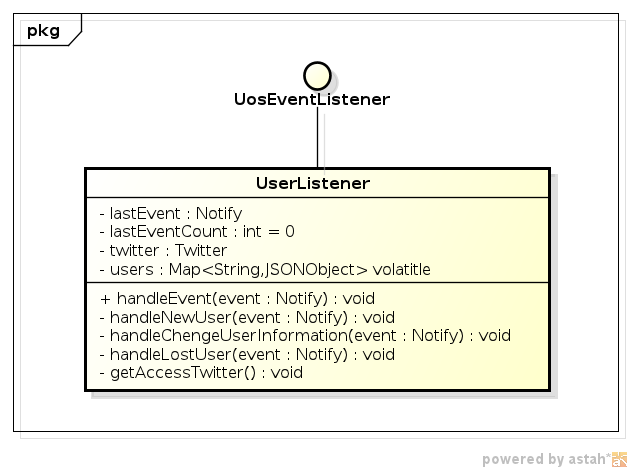
\includegraphics[scale=0.6]{figuras/5.Testes/diagrama-classe-user-listener.png}
		% 	\end{center}
		% 	\caption{Diagrama de Classe do \textit{listener} \textit{UserListener}.}
		% 	\label{fig:diagrama-userlistener}
		% \end{figure}

	% Basicamente, quando o \textit{UserListener} obtém os eventos do \textit{UserDriver}, ele envia mensagens pelo Twitter~\cite{twitter} para os usuários no ambiente, conforme o evento recebido. Para enviar as mensagens pelo Twitter foi utilizado a biblioteca \textit{twitter4j}~\cite{twitter4j}. A Figura~\ref{fig:diagrama-tweet} mostra o fluxo básico de execução do \textit{listener} e as mensagens padrões para cada tipo de evento recebido. 

	Basicamente, quando o \textit{UserListener} é inicializado ele obtém acesso ao twitter e se registra para escutar os eventos gerados pelo \textit{UserDriver}. Para cada evento obtido, ele envia mensagens pelo Twitter~\cite{twitter} para os usuários no ambiente. Para eventos de ``novo usuário detectado'' e ``usuário perdido'', ele envia mensagens de boas vindas e de despedidas respectivamente. Como mencionado na Seção~\ref{sec:modulo-integracao}, o \textit{UserDriver} também gera eventos de atualização dos dados dos usuários. Quando estes eventos são gerados, o \textit{UserListener} verifica se houve atualização na identidade do usuário e se o mesmo está a mais de uma hora no mesmo lugar. Caso esteja, ele envia mensagens aos usuários informando estes acontecimentos. Este fluxo de execução e as estruturas das mensagens enviadas são mostrados na Figura~\ref{fig:diagrama-tweet}. Para enviar as mensagens pelo Twitter foi utilizado a biblioteca \textit{twitter4j}~\cite{twitter4j}.

	\begin{figure}[hbt]
		\begin{center}
			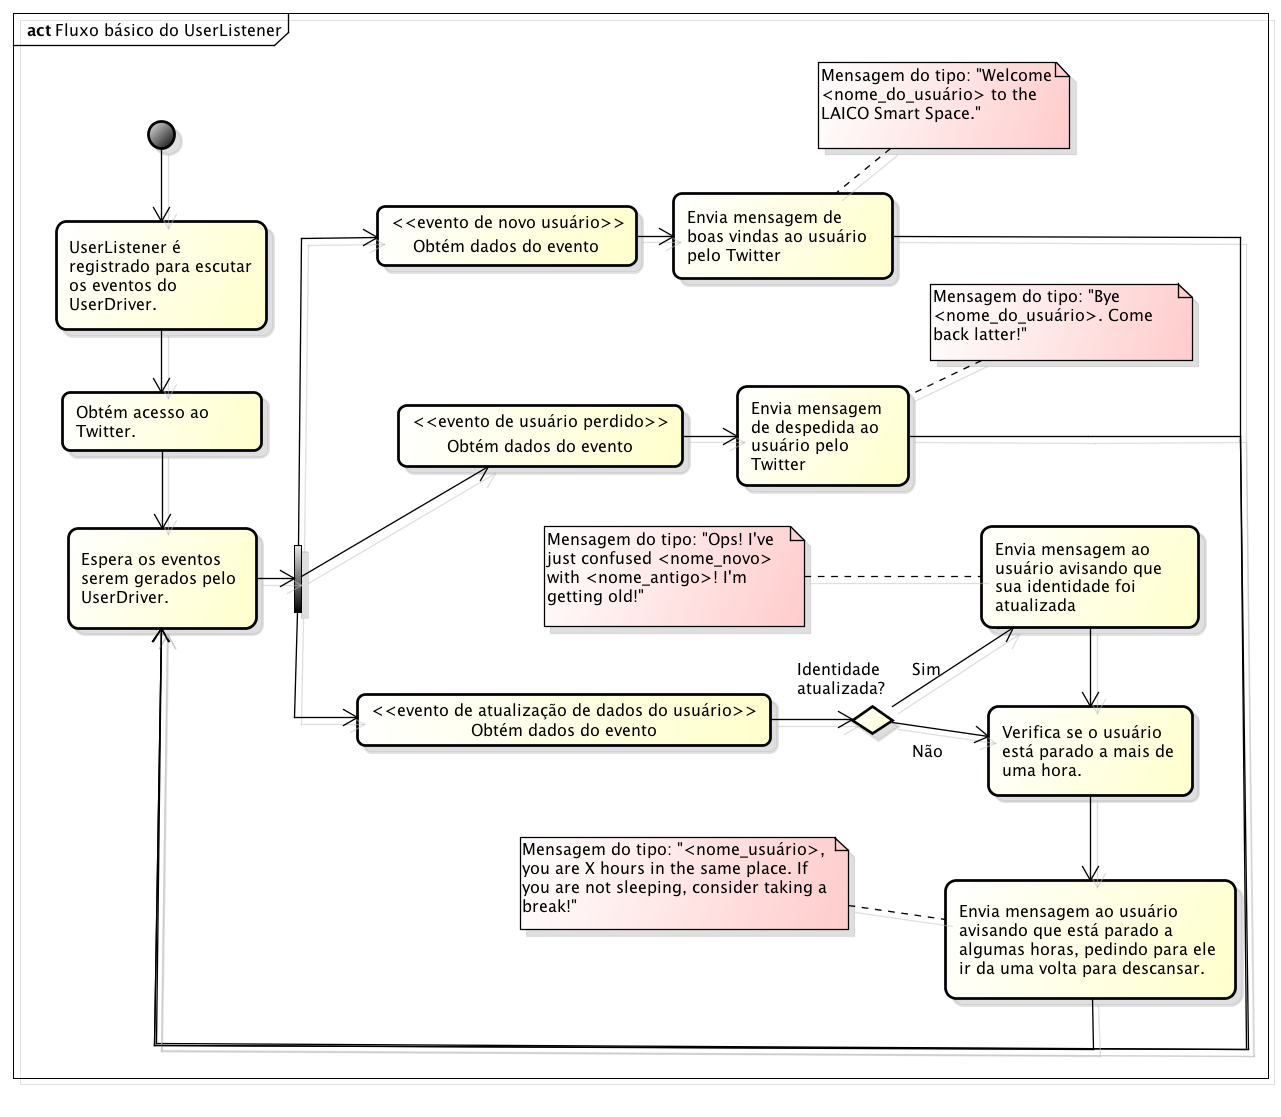
\includegraphics[scale=0.45]{figuras/5.Testes/diagrama-user-tweet.png}
		\end{center}
		\caption{Fluxo básico de execução do \textit{listener} \textit{UserListener}.}
		\label{fig:diagrama-tweet}
	\end{figure}

	Testes funcionais foram feitos com a aplicação mostrando que o \textit{driver} consegue
	obter os dados íntegros do Sistema TRUE e gerar os eventos de maneira praticamente
	instantânea. Algumas vezes as mensagens demoravam a chegar ao Twitter,
	geralmente nos horários de pico quando o Twitter operava próximo ao limite
	da sua capacidade. A Figura~\ref{fig:tweets} mostra as mensagens geradas
	pela aplicação em um teste funcional, onde Danilo, um usuário cadastrado,
	entra no ambiente senta em uma mesa com seu notebook permanecendo no mesmo
	lugar por mais de uma hora, e logo depois deixa o ambiente.

	\begin{figure}[hbt]
			\begin{center}
				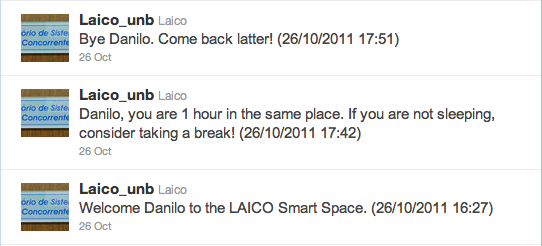
\includegraphics[scale=0.6]{figuras/5.Testes/tweets.png}
			\end{center}
			\caption{Exemplo das mensagens enviadas pelo Twitter aos usuários no ambiente.}
			\label{fig:tweets}
		\end{figure}	











